\subsection{Data logging}
\paragraph{}
For the first part of this image processing, we had to collect images.
So first we went into the environment in which the robot was going to evolve.

\begin{figure}[h!]
    \begin{center}
        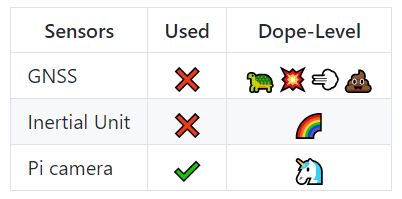
\includegraphics[scale=0.3]{Images/Sensors.png}
    \end{center}
    \caption{collecting data}
    \label{fig:capture}
\end{figure}

\subsection{pre binarization treatment}
\paragraph{}
In this part, we first had to perform a pre-binarization treatment in order to reduce post-binarization noise.
So we used a Gaussian filter to blur the image.

\subsection{binarization}
\paragraph{}
Since the line we wanted to mark is white. An effective treatment is simply to switch to grey level. 
So for binarization, we switch the image to a grey level and threshold for a grey level that we have determined empirically.

\subsection{post binarization treatment}
\paragraph{}
In this part we performed a morphological treatment. There was still a lot of noise after binarization. So we made an opening. 
With a kernel in the shape of a rectangle (since it was the most efficient for this treatment).
At the end of this treatment we obtain a well defined line which crosses the screen.

\subsection{find the center of the line}
\paragraph{}
In this last part, the contours are marked using a gradient method. Then the contours are sorted from the smallest to the largest.
We recover the largest contour.
And we recover the coordinates of the barycentre of the contour.
Then the error is the difference between the center of the image and the coordinates of the pixel.
